%%%%%%%%%%%%%%%%%%%%%%%%%%%%%%%%%%%%%%%%%%%%%%
%% Set up
%%%%%%%%%%%%%%%%%%%%%%%%%%%%%%%%%%%%%%%%%%%%%%
\documentclass{beamer}
\usepackage[utf8]{inputenc}
\usepackage[T1]{fontenc}
\usepackage{lmodern}
\usepackage{hyperref}
\usepackage{tikz}
\graphicspath{{/home/paul/Dropbox/MARES_PhD/jointprod_study/data/figure/}}

\AtBeginSection{\frame{\sectionpage}}
\addtocounter{framenumber}{-1}

%%%%%%%%%%%%%%%%%%%%%%%%%%%%%%%%%%%%%%%%%%%%%%
\title{Modelling spatio-temporal dynamics \\ 
	of Celtic Sea fisheries}   
\author{Paul Dolder, Jim Thorson \& Cóilín Minto}
\date{February 9, 2017} 
%%%%%%%%%%%%%%%%%%%%%%%%%%%%%%%%%%%%%%%%%%%%%%
\begin{document}
%%%%%%%%%%%%%%%%%%%%%%%%%%%%%%%%%%%%%%%%%%%%%%%
\frame{\titlepage} 
\frame{\frametitle{Table of contents}\tableofcontents} 
%%%%%%%%%%%%%%%%%%%%%%%%%%%%%%%%%%%%%%%%%%%%%%%%
\section{Objectives} 
%%%%%%%%%%%%%%%%%%%%%%%%%%%%%%%%%%%%%%%%%%%%%%%%
\frame{\frametitle{Goals for study} 
\begin{enumerate}
\setlength\itemsep{2em}
\item Evaluate inter-species dynamics of main commercial fish populations in
	the Celtic Sea 
\item Explore strength of interdependence of fisheries on the different species
	(as an insight into the ability to spatially separate catches of
	species \textit{x} from species \textit{y})
\item Make efficient use of (and combine) the various surveys that have been
	undertaken in IE, FR, UK in past 20-odd years.
\end{enumerate}

}

%%%%%%%%%%%%%%%%%%%%%%%%%%%%%%%%%%%%%%%%%%%%%%%%
\frame{\frametitle{Expected outcomes}
\begin{enumerate}
\setlength\itemsep{2em}
	\item A useful index of abundance for the species/species groups
		following treatment for the irregular spatial survey coverage
		and sampling methods
	\item A measure of dependence of the different species in space and time.
	\item Insight into the spatio-temporal dynamics of the individual
		species as a pre-cursor to exploring how spatial abundance
		estimates can be used for fleet dynamics models.
\end{enumerate}
}

%%%%%%%%%%%%%%%%%%%%%%%%%%%%%%%%%%%%%%%%%%%%%%%%
\section{Methods} 
%%%%%%%%%%%%%%%%%%%%%%%%%%%%%%%%%%%%%%%%%%%%%%%%
\frame{\frametitle{Modelling framework} 
\begin{itemize}
\setlength\itemsep{1em}
	\item Used \textbf{VAST} (Vector-Autoregressive Spatio-temporal) model
		developed by Jim Thorson @ NOAA, NWFSC, Seattle.
	\item Spent approx. 5 weeks in Seattle over the summer, based at SAFS, UW
\end{itemize}
\begin{tikzpicture}
\node (img1) {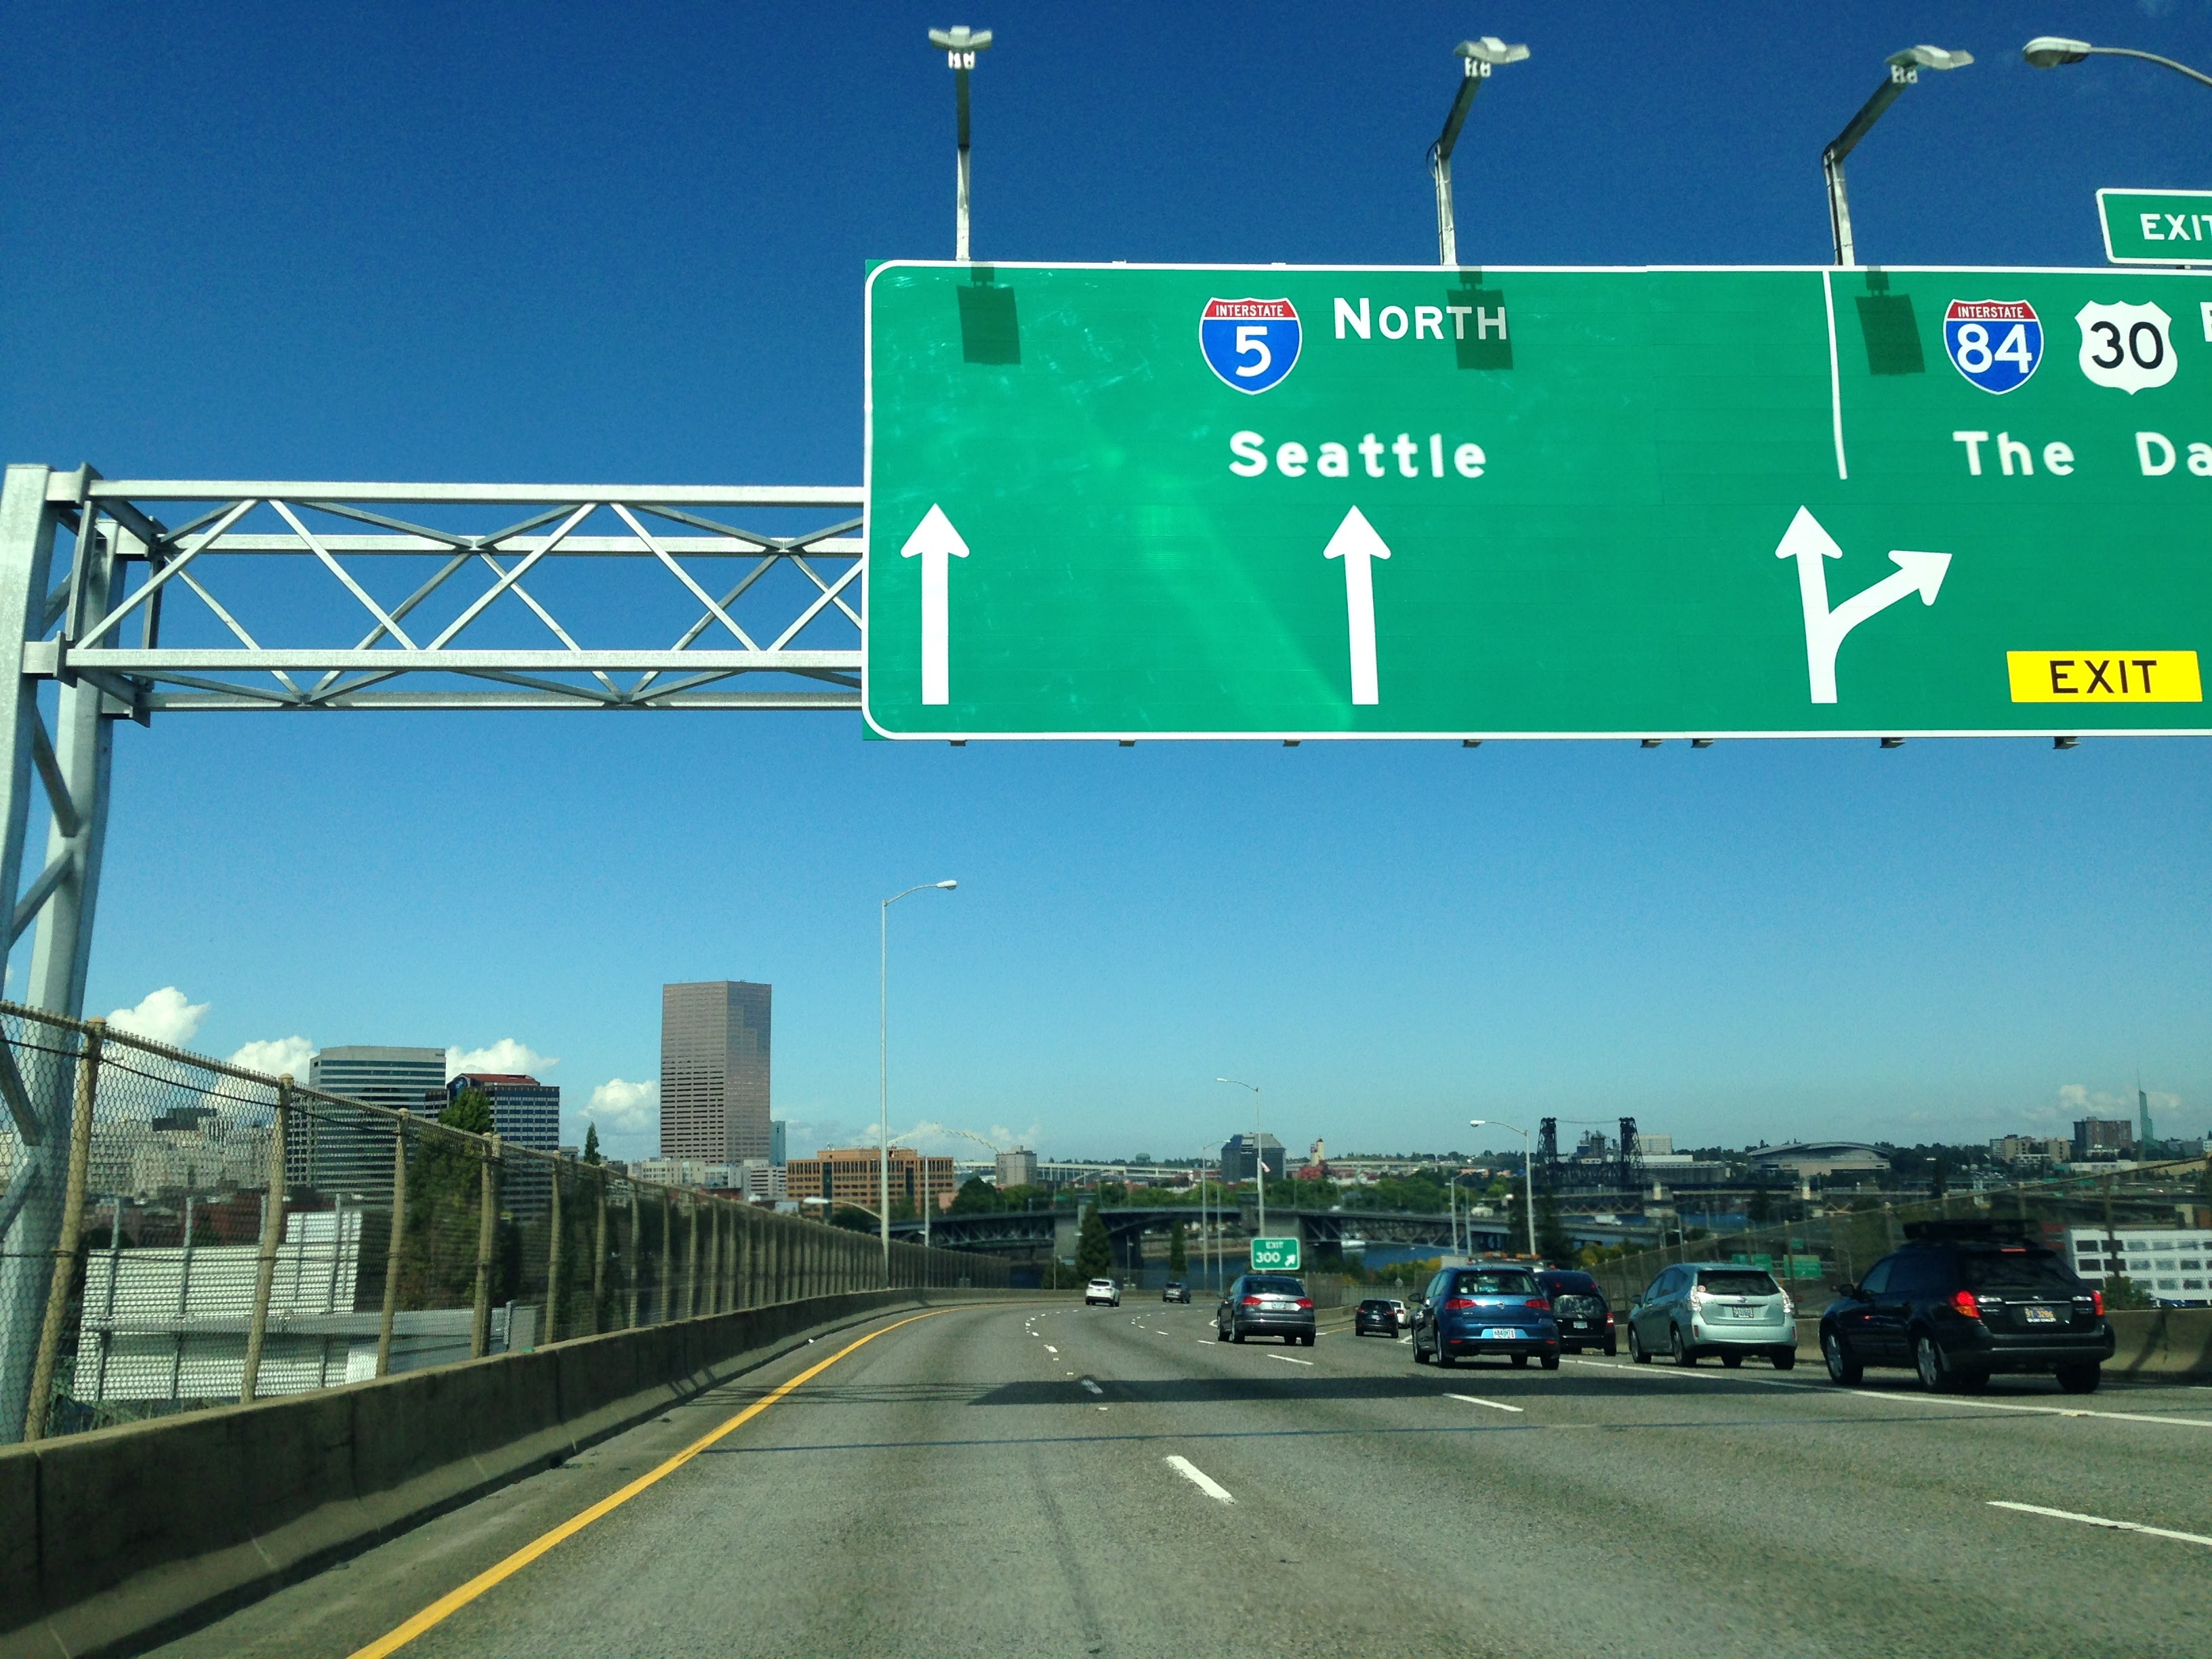
\includegraphics[width = 4cm, height =
	3cm]
	{/home/paul/Dropbox/MARES_PhD/jointprod_study/docs/paper_headers/IMG_1941}};
\node (img2) at (img1.south east)[xshift = 4em] {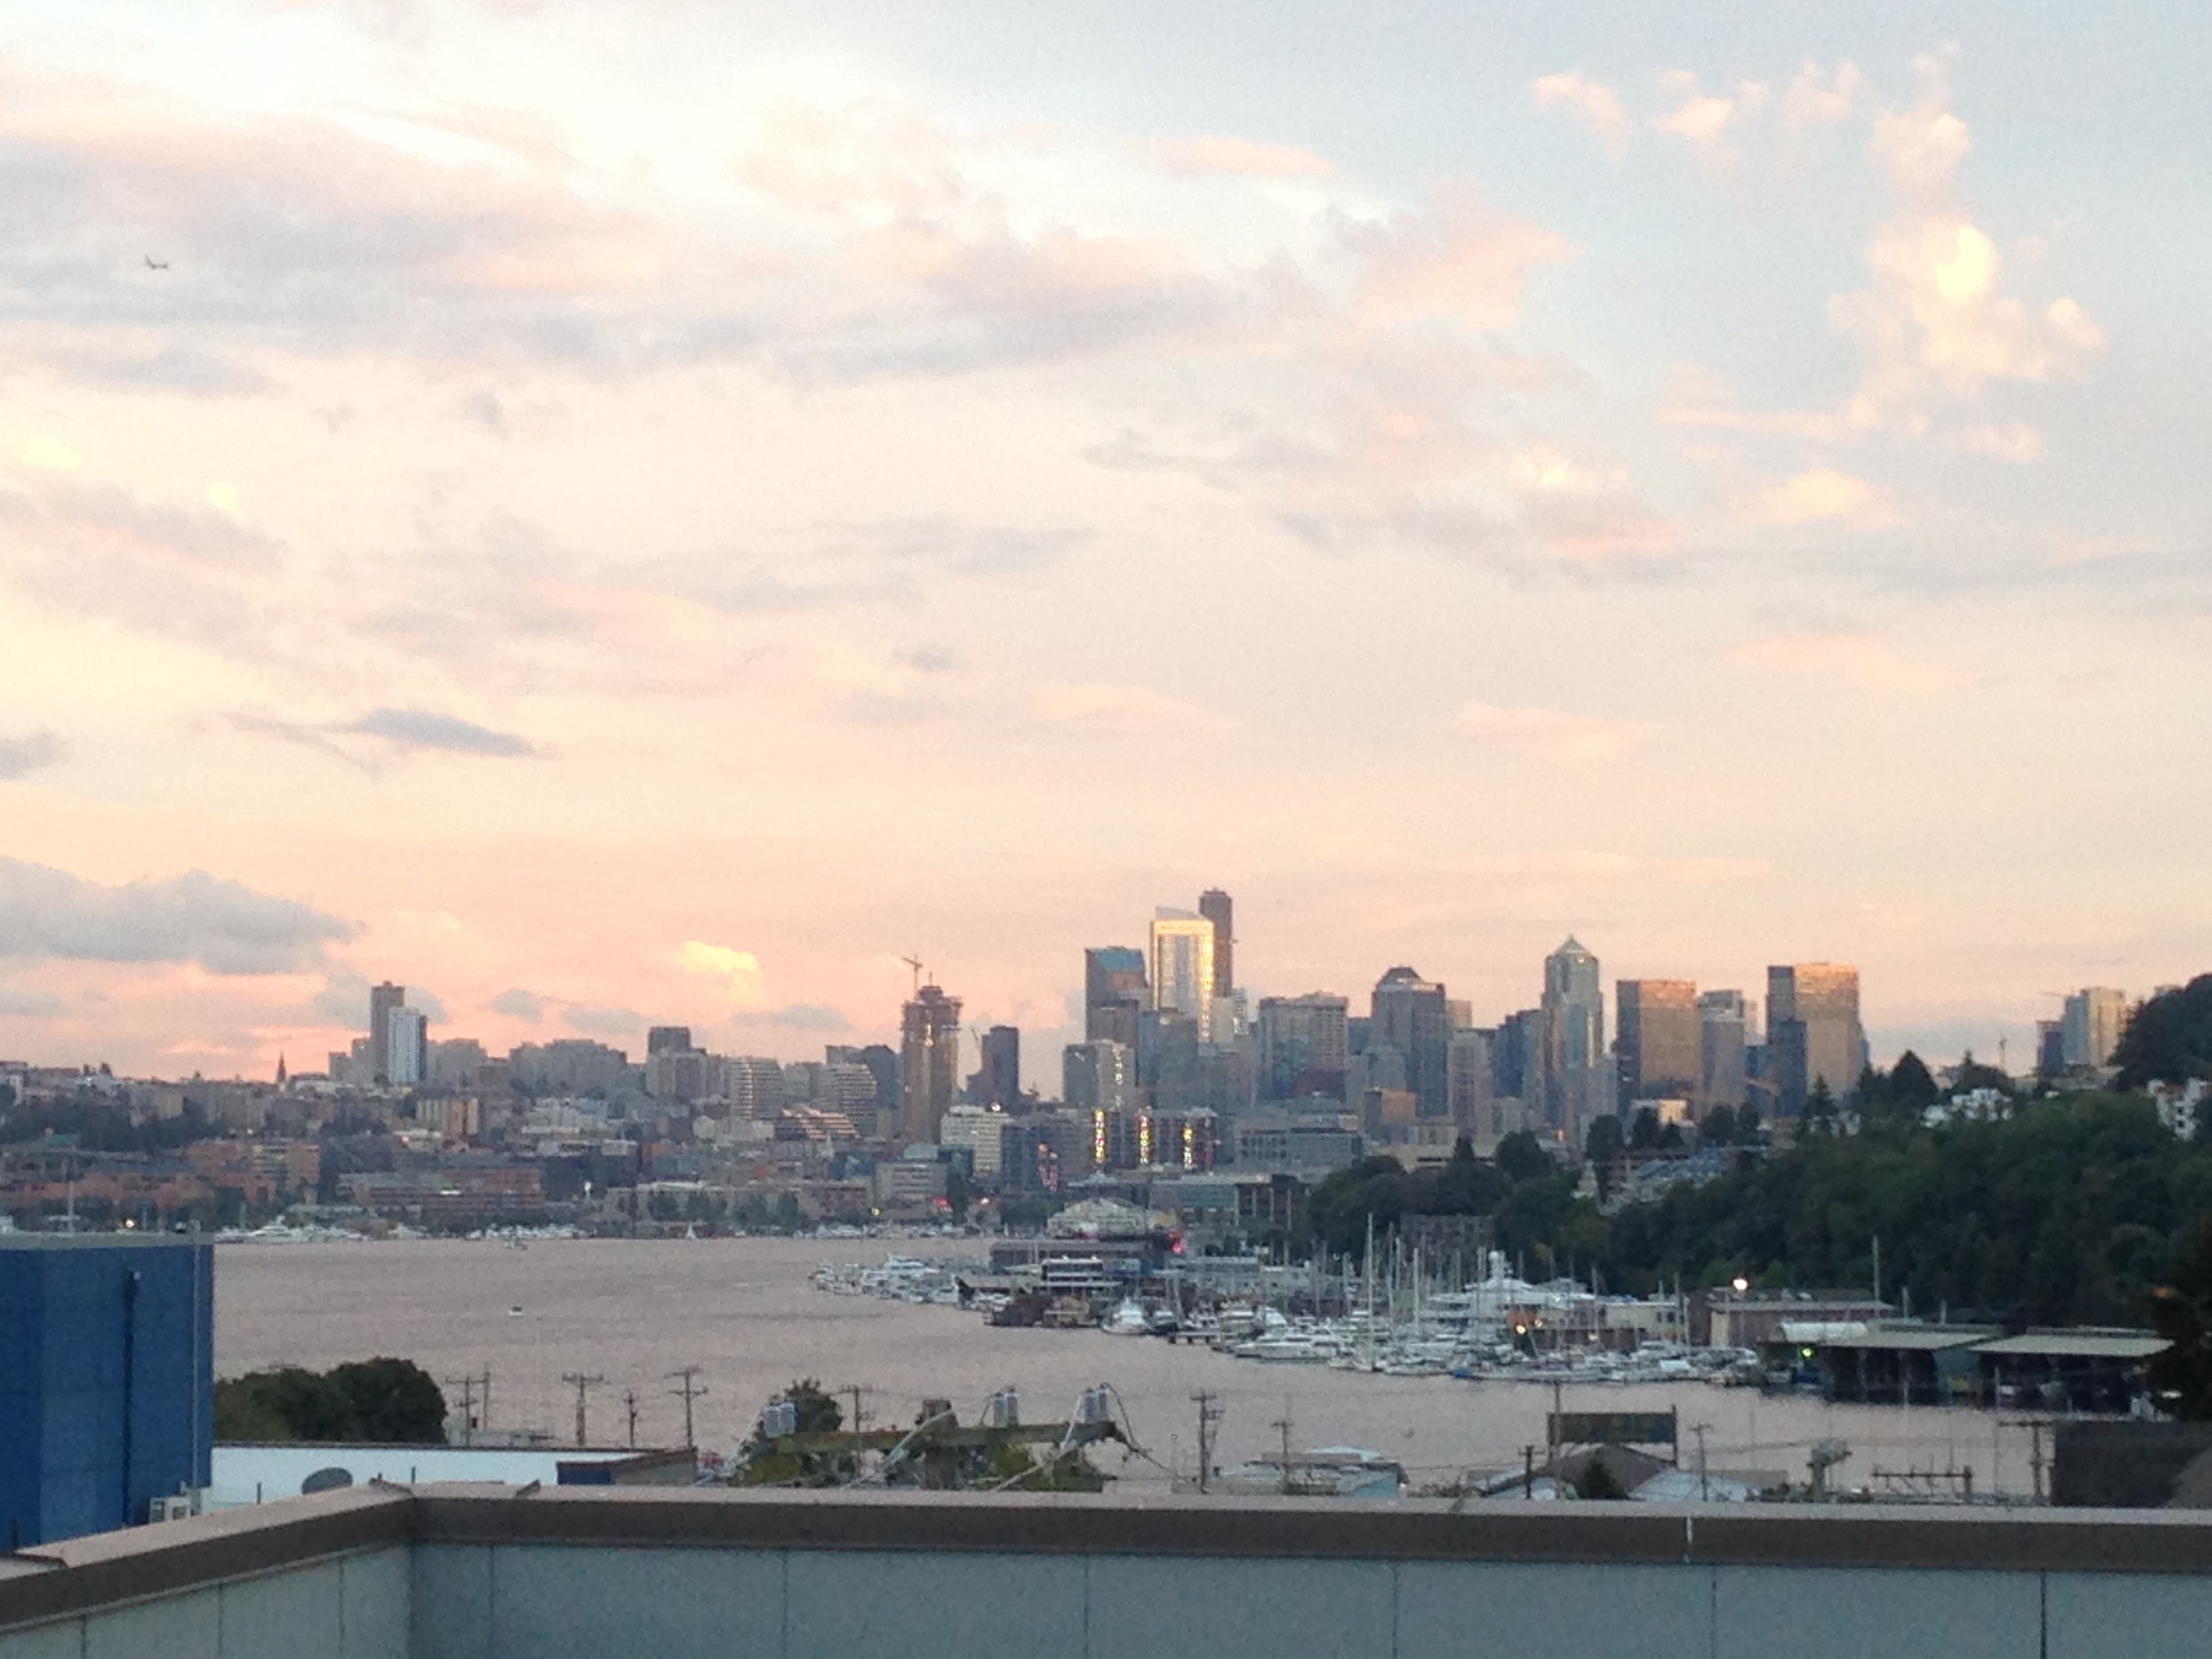
\includegraphics[width = 4cm, height =
	3cm] {/home/paul/Dropbox/MARES_PhD/jointprod_study/docs/paper_headers/IMG_1625}};
\node (img3) at (img2.south east)[xshift = 4em] {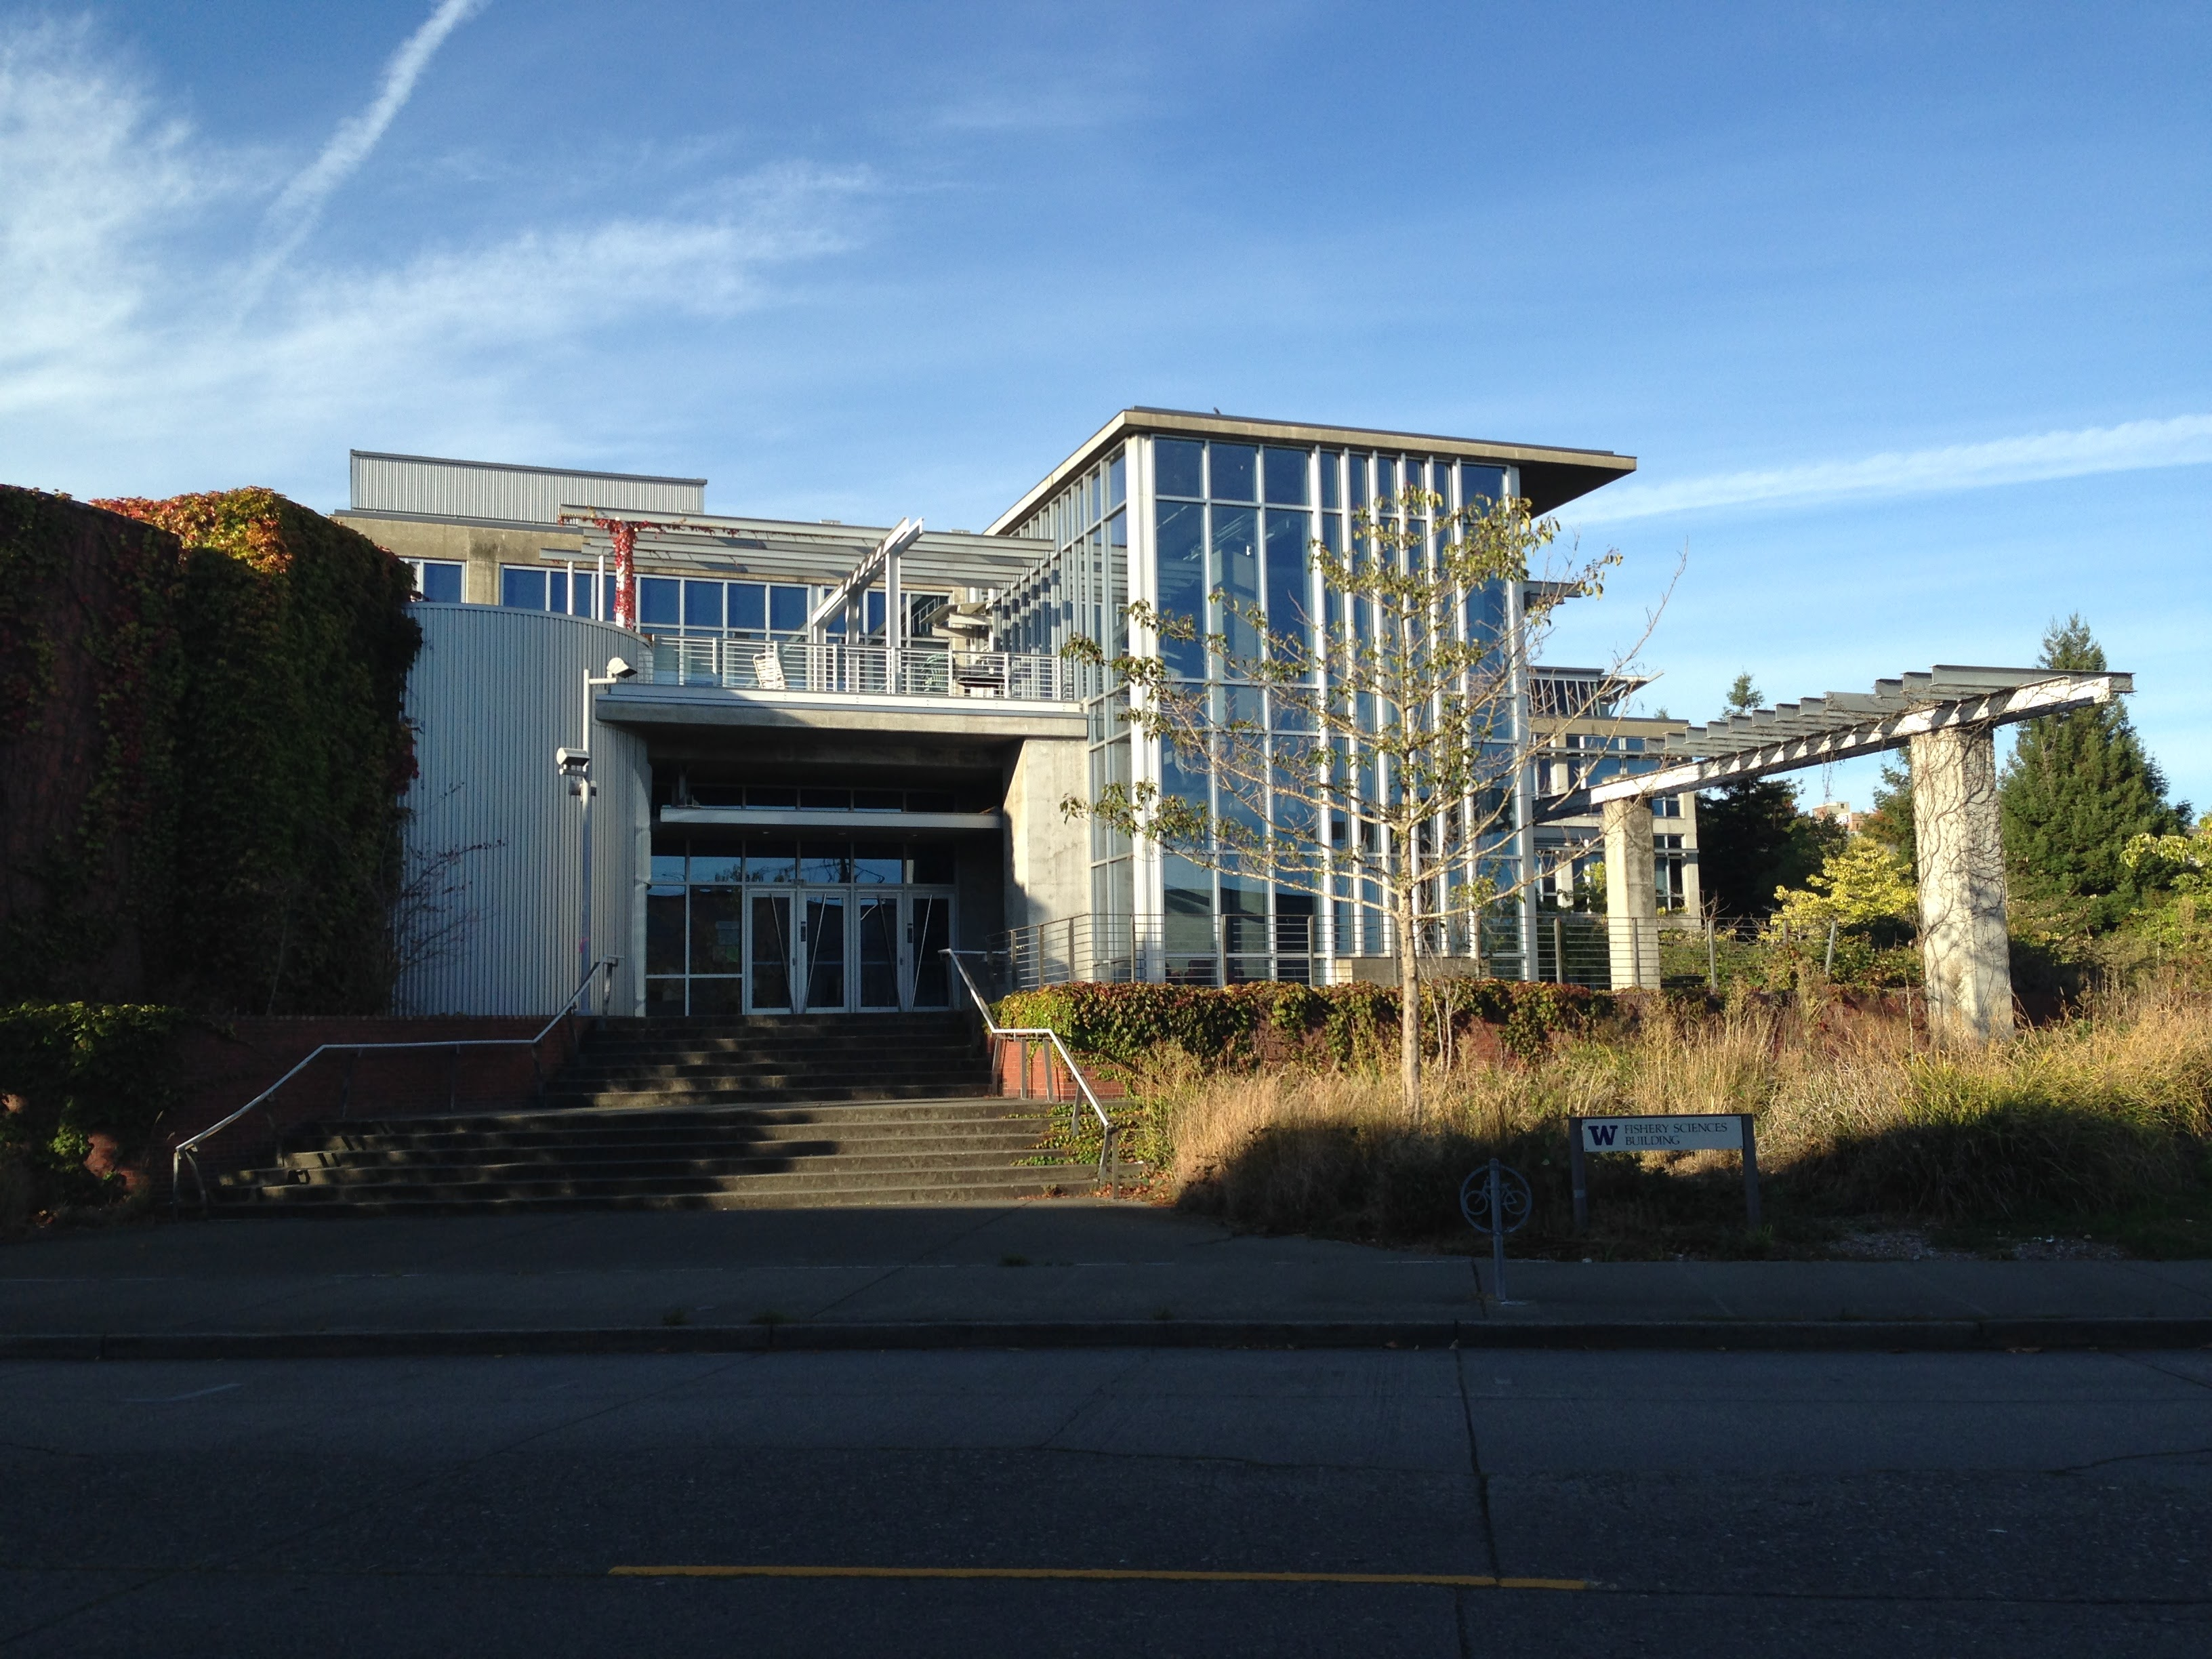
\includegraphics[width = 4cm, height =
	3cm] {/home/paul/Dropbox/MARES_PhD/jointprod_study/docs/paper_headers/IMG_2052}};
\end{tikzpicture}
}

%%%%%%%%%%%%%%%%%%%%%%%%%%%%%%%%%%%%%%%%%%%%%%

\frame{\frametitle{Modelling framework}

\begin{itemize}
	\item VAST implements a spatio-temporal delta-generalised linear mixed model
		taking account of correlations among multiple species / size
		classes.
	\item Estimates spatio-temporal variation in density with spatial point
		data.
	\item VAST builds from several developments by Jim and others in using
		model-based geostatistical methods. 
	\item It can be found and installed as an R package @
		\url{https://github.com/james-thorson/VAST}
	\end{itemize}
}

%%%%%%%%%%%%%%%%%%%%%%%%%%%%%%%%%%%%%%%%%%%%%%%%
\frame{\frametitle{Modelling framework} 

Numerous publications documenting development of elements of the modelling framework:

\begin{tikzpicture}
\node (img1) {\includegraphics[width = 10cm]{/home/paul/Dropbox/MARES_PhD/jointprod_study/docs/paper_headers/Selection_012}};
\pause
\node (img2) at (img1.south) {\includegraphics[width = 10cm]{/home/paul/Dropbox/MARES_PhD/jointprod_study/docs/paper_headers/Selection_013}};
\pause
\node (img3) at (img2.north) {\includegraphics[width = 10cm]{/home/paul/Dropbox/MARES_PhD/jointprod_study/docs/paper_headers/Selection_011}};
\pause
\node (img4) at (img3.south) {\includegraphics[width = 10cm]{/home/paul/Dropbox/MARES_PhD/jointprod_study/docs/paper_headers/Selection_014}};
\pause
\node (img5) at (img4.north) {\includegraphics[width = 10cm]{/home/paul/Dropbox/MARES_PhD/jointprod_study/docs/paper_headers/Selection_010}};

\end{tikzpicture}

}

%%%%%%%%%%%%%%%%%%%%%%%%%%%%%%%%%%%%%%%%%%%%%%%%
\frame{\frametitle{Key properties of model} 
\begin{enumerate}
\setlength\itemsep{1em}
	\item Two-stage "delta-"GLMM
		\begin{itemize}
			\item logit-link linear predictor for \textit{encounter
				probability}
			\item log or gamma link linear predictor for \textit{catch rate}
		\end{itemize}
	\item Gaussian Markov Random Field (GMRF) process to model
		spatio-temporal variation in abundance as a random effect
		\begin{itemize}
			\item Includes covariance matrices to describe
				encounter probability \& catch rate among locations
			\item Includes covariance matrices to describe
				encounter probability \& catch rate among
				species(group)
			\item covariance modelled with a matérn correlation
				structure [decays smoothly over space/time] -
				distance estimated within model
		\end{itemize}
\end{enumerate} 
}

%%%%%%%%%%%%%%%%%%%%%%%%%%%%%%%%%%%%%%%%%%%%%%
\frame{\frametitle{key properties of model}
	\begin{itemize}
	\item Spatial correlation function - range and shape param estimated 
	\end{itemize}
	\centering
\includegraphics[width = 8cm]{/home/paul/Dropbox/MARES_PhD/Geostatistics/Sim_data/plots/Matern_example}
}

%%%%%%%%%%%%%%%%%%%%%
\frame{\frametitle{Key properties of model}
\begin{enumerate}
\setlength\itemsep{1em}
		\setcounter{enumi}{2}
	\item Covariance among species is represented by loading factors
		following a factor-analysis decomposition.\\ \hspace{1cm}
		\textgreater \textgreater \hspace{1cm} reduces dimensionality
		of the model
	\item Can incorporate fixed or random vessel effects as well as covariates
		for spatial predictions (e.g. habitat, depth).
	\item Input to the model is the point data for catches (in weight) per
		species, per station and an estimate of swept area. Seasonal
		variation can also be incorporated in later versions of
		software.
\end{enumerate}

}

%%%%%%%%%%%%%%%%%%%%%%%%%%%%%%%%%%%%%%%%%%%%%%%%
\frame{\frametitle{Model implementation} 
\begin{enumerate}
\setlength\itemsep{1em}
	\item Model uses INLA R package to find (a user defined number of) spatial knots
		reflecting the spatial distribution of the data
	\item Parameter estimation for fixed effects done via Maximum
		Likelihood Estimation (MLE) in Template Model Builder (TMB) via the
		Laplace approximation. The TMB code is auto-generated by the R
		package.
	\item Have been fitting using the super-computer at ICHEC (Irish Centre for High End Computing)
		\begin{itemize}
			\item low level parallelisation on 24 cores, access to
				lots of memory
			\item Still takes long runtimes (~ 2 days)
				\begin{flushright}
				\includegraphics[width = 3cm]{/home/paul/Dropbox/MARES_PhD/jointprod_study/docs/paper_headers/ichec_logo}
				
\includegraphics[width =2cm]{/home/paul/Dropbox/MARES_PhD/jointprod_study/docs/paper_headers/IMG_2068}
			\end{flushright}
		\end{itemize}
\end{enumerate}
}


%%%%%%%%%%%%%%%%%%%%%%%%%%%%%%%%%%%%%%%%%%%%%%%%
\section{Data exploration} 
%%%%%%%%%%%%%%%%%%%%%%%%%%%%%%%%%%%%%%%%%%%%%%%%
\frame{\frametitle{Available survey data} 
\begin{itemize}
\setlength\itemsep{2em}
	\item Collated available survey data from both ICES Datras (IE-IGFS,
		FR-EVHOE) and Cefas data (WCGFS, Q4SWIBTS, Q1SWBEAM, NWGFS,
		CARLHELMAR).
	\item Selected catch records for gadoids (cod, haddock, whiting, hake),
		flatfish (plaice, sole) and shelf (anglerfishes (2 spp.),
		megrims).
	\item Processed catch data to estimate biomass per swept area per tow
		for 2 size classes per species: juveniles (\textless MCRS) and adults
		(\textgreater MCRS).
\end{itemize}
}

%%%%%%%%%%%%%%%%%%%%%%%%%%%%%%%%%%%%%%%%%%%%%%%%
\frame{\frametitle{Processing steps}

Station data:
\begin{enumerate}
	\item Retain only valid hauls, removing any with outlier tow distances
	\item Estimate swept area for tows based on gear and distance towed.
		\begin{itemize}
		\item For beam trawls: fixed width * distance * CF
		\item For otter trawls: Doorspread * distance * CF
		\end{itemize}
		\end{enumerate}

Haul data:
\begin{enumerate}
	\item Clean up any outliers (EVHOE 2.5m whiting!)
	\begin{center}
	\includegraphics[width=2cm]{/home/paul/Dropbox/MARES_PhD/jointprod_study/docs/paper_headers/thalasa}
	\includegraphics[width=3cm]{/home/paul/Dropbox/MARES_PhD/jointprod_study/docs/paper_headers/fish}
	\end{center}
	\item Estimate length weight relationships (from EVHOE data) using a
		GLM
		\begin{itemize}
			\item Use to raise numbers at length to weight
			\item Split catch between \textless MCRS and
				\textgreater MCRS
		\end{itemize}
	\end{enumerate}
}

%%%%%%%%%%%%%%%%%%%%%%%%%%%%%%%%%%%%%%%%%%%%%%%%%
\frame{\frametitle {Survey temporal coverage}
\includegraphics[height = 8cm]{Survey_by_year-1}
}
%%%%%%%%%%%%%%%%%%%%%%%%%%%%%%%%%%%%%%%%%%%%%%%%
\frame{\frametitle {Survey temporal coverage 2}
\includegraphics[height = 8cm]{Survey_by_month-1}
}
%%%%%%%%%%%%%%%%%%%%%%%%%%%%%%%%%%%%%%%%%%%%%%%%
\frame{\frametitle {Survey temporal coverage 3}
\includegraphics[height = 8cm]{Survey_effort_by_year-1}
}
%%%%%%%%%%%%%%%%%%%%%%%%%%%%%%%%%%%%%%%%%%%%%%%%
\frame{\frametitle {Survey spatial coverage 1}
\includegraphics[height = 6cm]{Survey_Spatial_extent-1}
}
%%%%%%%%%%%%%%%%%%%%%%%%%%%%%%%%%%%%%%%%%%%%%%%%
\frame{\frametitle {Survey spatial coverage 2}
\includegraphics[height = 6cm]{Survey_Spatial_extent-2}
}

%%%%%%%%%%%%%%%%%%%%%%%%%%%%%%%%%%%%%%%%%%%%%%%%
\frame{\frametitle {Survey spatial coverage 3}
\includegraphics[height = 9cm]{Survey_locations-1}
}

\frame{\frametitle {Swept Area}
	\centering
\includegraphics[width = 6cm]{Survey_swept_area-1}
\includegraphics[width = 6cm]{Survey_swept_area-2}

}

%%%%%%%%%%%%%%%%%%%%%%%%%%%%%%%%%%%%%%%%%%%%%%%%
\frame{\frametitle {Length weight relationships}
	\centering
\includegraphics[width = 8cm]{Predictions2-1}
}

%%%%%%%%%%%%%%%%%%%%%%%%%%%%%%%%%%%%%%%%%%%%%%%%
\frame{\frametitle {Raw CPUE}
	\centering
\includegraphics[width = 12cm]{CPUE-1}
}

%%%%%%%%%%%%%%%%%%%%%%%%%%%%%%%%%%%%%%%%%%%%%%%%
\frame{\frametitle {Survey catches - example adult cod}
	\centering
\includegraphics[width = 12cm]{Survey_catches-1}
}

%%%%%%%%%%%%%%%%%%%%%%%%%%%%%%%%%%%%%%%%%%%%%%%%
\frame{\frametitle {Survey catches - example juvenile cod}
	\centering
\includegraphics[width = 12cm]{Survey_catches-2}
}


%%%%%%%%%%%%%%%%%%%%%%%%%%%%%%%%%%%%%%%%%%%%%%%%
\section{Preliminary outputs and conclusions} 
%%%%%%%%%%%%%%%%%%%%%%%%%%%%%%%%%%%%%%%%%%%%%%%%

\frame{\frametitle{Model setup}

\begin{itemize}
		\setlength\itemsep{1em}
	\item Years: \hspace{2cm}  1990 - 2015
	\item Species/Groups:  \hspace{0.35cm} 18
	\item Factors:  \hspace{1.7cm} 10
	\item Knots: \hspace{1.9cm} 250 (so far)
	\item logit for encounter prob. and gamma distribution on positive
		catches
	\item Covariates:
		\begin{itemize}
			\item Gears as fixed effects: 7
			\item Substrate classifications (6) and
				depth (1)
		\end{itemize}
	\item 1522 total fixed effects and 143 640 random effects
\end{itemize}

}

%%%%%%%%%%%%%%%%%%%%%%%%%%%%%%%%%%%%%%%%%%%%%%%
\frame{\frametitle{Model checking}
\includegraphics[width=5cm]{/home/paul/Dropbox/MARES_PhD/jointprod_study/results/2017-02-07_RUN_FULL/Q-Q_plot}
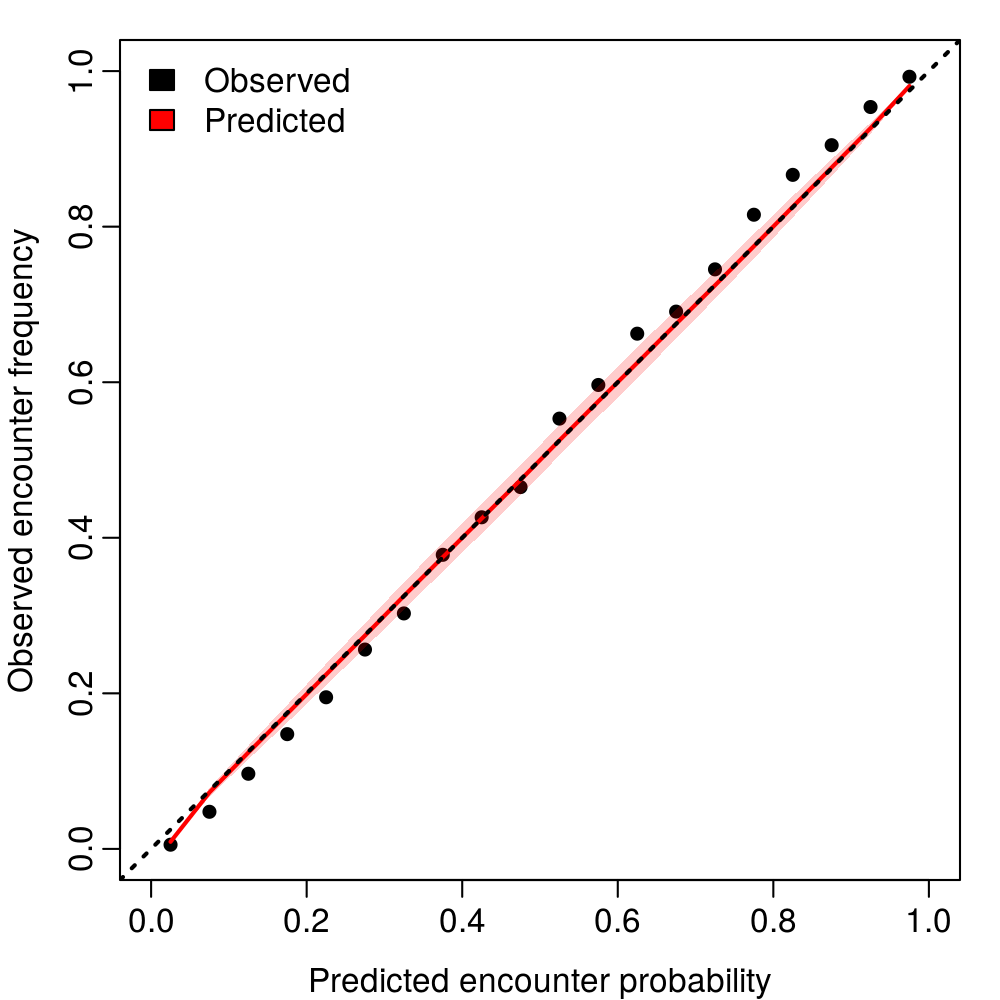
\includegraphics[width=4.78cm]{/home/paul/Dropbox/MARES_PhD/jointprod_study/results/2017-02-07_RUN_FULL/Diag--Encounter_prob}
}

%%%%%%%%%%%%%%%%%%%%%%%%%%%%%%%%%%%%%%%%%%%%%%%%
\frame{\frametitle{Anisotropic effect}
\centering
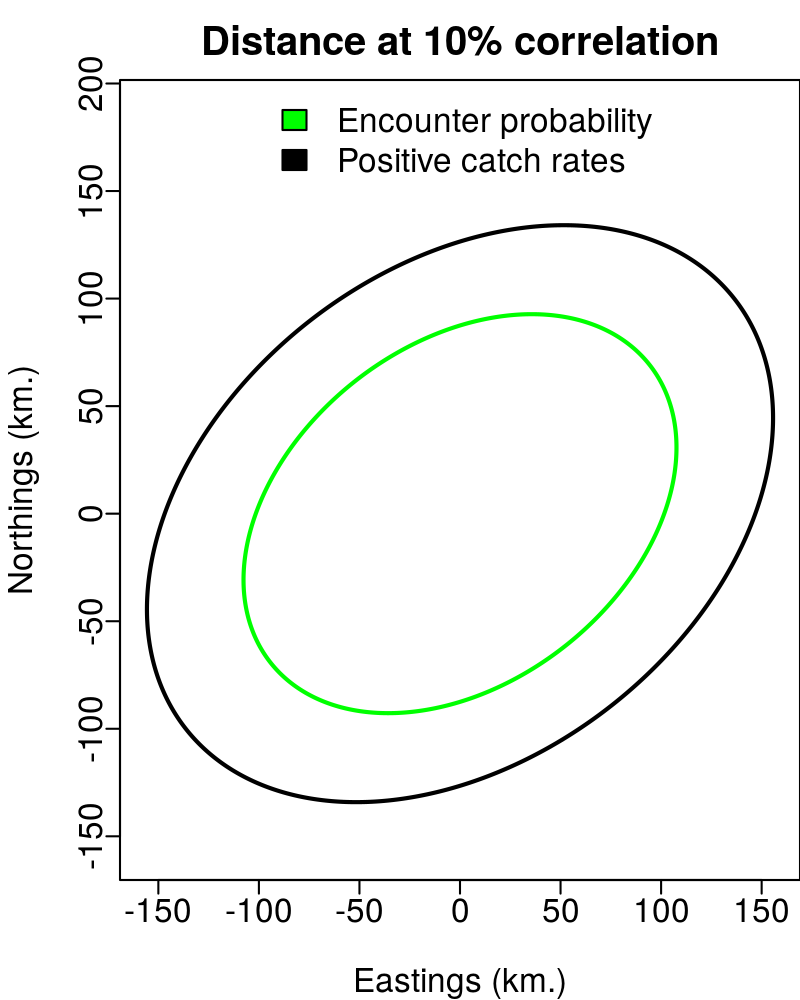
\includegraphics[width =6cm]{/home/paul/Dropbox/MARES_PhD/jointprod_study/results/2017-02-07_RUN_FULL/Aniso}
}

%%%%%%%%%%%%%%%%%%%%%%%%%%%%%%%%%%%%%%%%%%%%%%%
\frame{\frametitle{Gear effect - needs work to understand}
	\centering
\includegraphics[width=5.5cm]{/home/paul/Dropbox/MARES_PhD/jointprod_study/results/2017-02-07_RUN_FULL/Gear_effects_ecounter}
\includegraphics[width=5.5cm]{/home/paul/Dropbox/MARES_PhD/jointprod_study/results/2017-02-07_RUN_FULL/Gear_effects_catch}
}

%%%%%%%%%%%%%%%%%%%%%%%%%%%%%%%%%%%%%%%%%%%%%%%
\frame{\frametitle{Species-group Covariances / Correlations}
	\centering
\includegraphics[width = 9.5cm]{/home/paul/Dropbox/MARES_PhD/jointprod_study/results/2017-02-04_RUN_FULL/Spatio-temporal_covariances--Analytic}
}


%%%%%%%%%%%%%%%%%%%%%%%%%%%%%%%%%%%%%%%%%%%%%%%%
\frame{\frametitle{Factor loadings - Spatio-temporal catch rates} 
	\centering
\includegraphics[width=5cm]{/home/paul/Dropbox/MARES_PhD/jointprod_study/results/2016-12-20_RUN_SIMPLE_BIG/Factor_loadings--Epsilon2}
}

%%%%%%%%%%%%%%%%%%%%%%%%%%%%%%%%%%%%%%%%%%%%%%%%
\frame{\frametitle{Indices} 
	\centering
\includegraphics[width = 8cm]{/home/paul/Dropbox/MARES_PhD/jointprod_study/results/2017-02-04_RUN_FULL/Index}
}

%%%%%%%%%%%%%%%%%%%%%%%%%%%%%%%%%%%%%%%%%%%%%%%%
\frame{\frametitle{Indices - Relative vs Relative SSB from assessment} 
	\centering
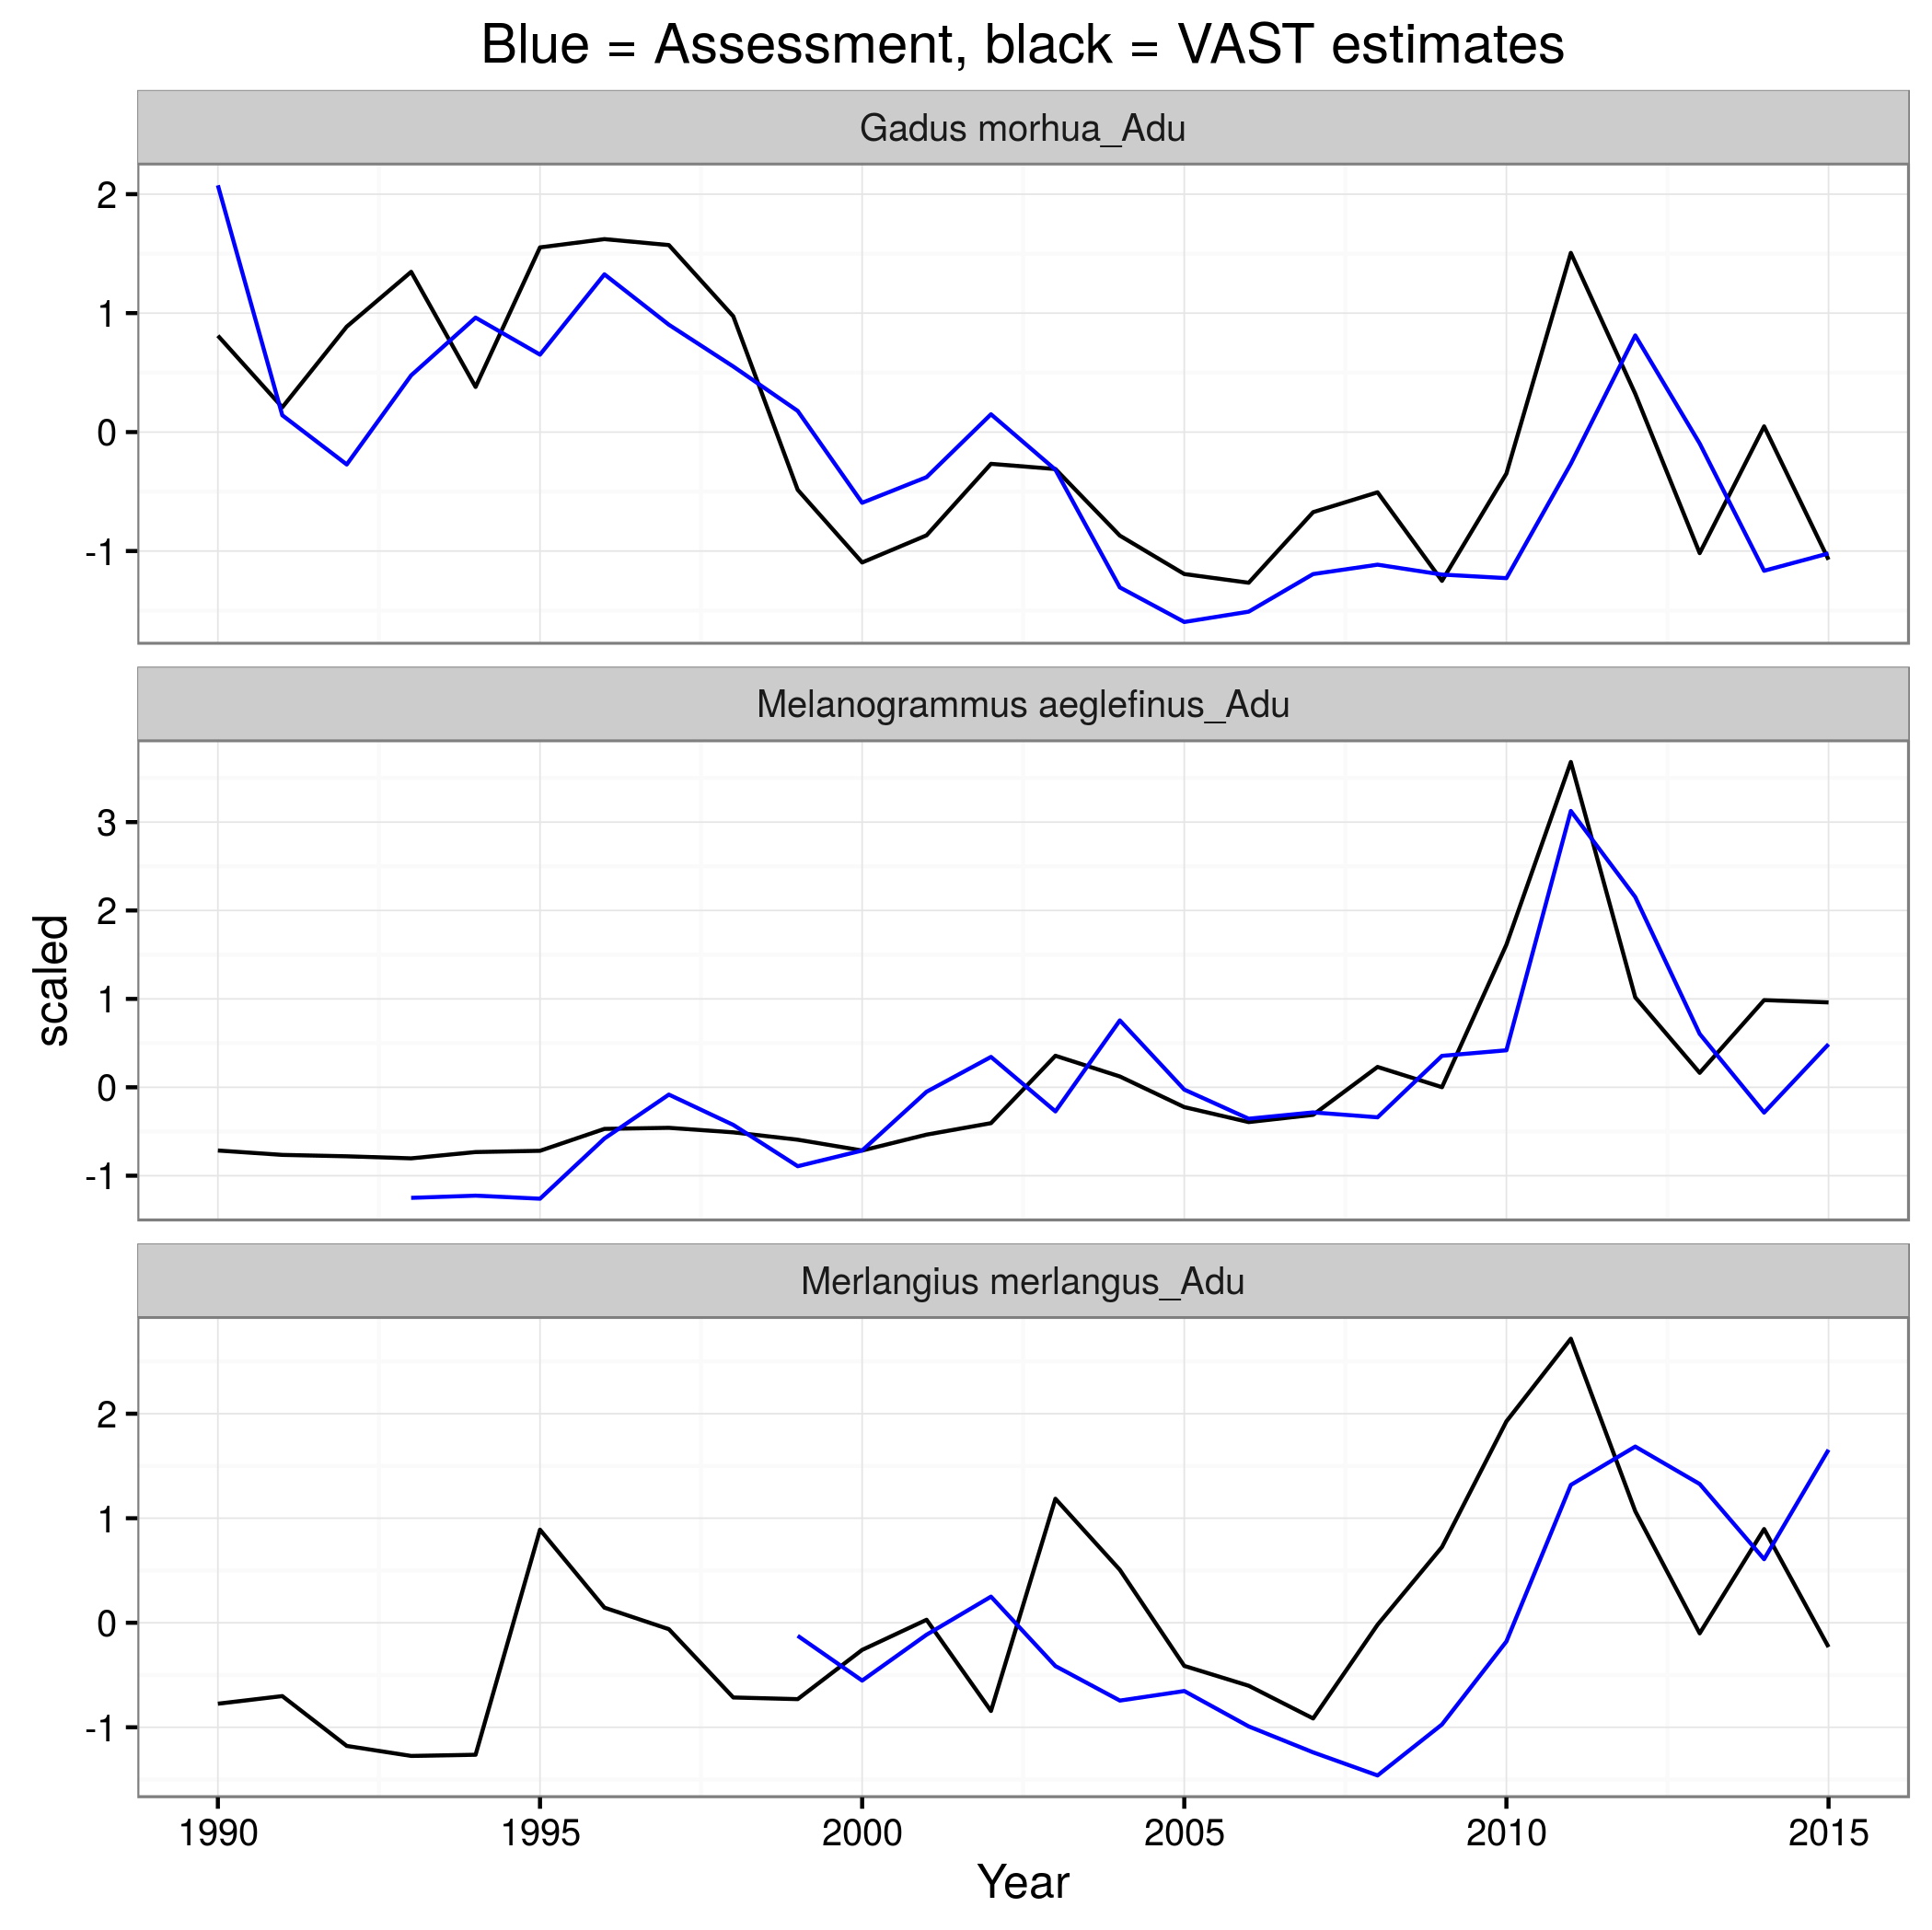
\includegraphics[width =8cm]{/home/paul/Dropbox/MARES_PhD/jointprod_study/docs/paper_headers/RealativeIndexVRelativeAssessSSB}
}

%%%%%%%%%%%%%%%%%%%%%%%%%%%%%%%%%%%%%%%%%%%%%%%%
\frame{\frametitle{Spatial densities - Adult cod}
	\centering
\includegraphics[width=10cm]{/home/paul/Dropbox/MARES_PhD/jointprod_study/results/2017-02-04_RUN_FULL/Field_Dens--Gadus_morhua_Adu}
}

\frame{\frametitle{Spatial densities - Juvenile cod}
	\centering
\includegraphics[width=10cm]{/home/paul/Dropbox/MARES_PhD/jointprod_study/results/2017-02-04_RUN_FULL/Field_Dens--Gadus_morhua_Juv}
}

%%%%%%%%%%%%%%%%%%%%%%%%%%%%%%%%%%%%%%%%%%%%

\frame{\frametitle{Thoughts on outputs}
	\begin{itemize}
		\setlength\itemsep{2em}
		\item Fully model-based geo statistical method incorporating
			spatial and temporal correlations within and across
			species
		\item Strong correlations within groups (gadoids, flats, shelf)
			indicating may be spatially difficult to separate
			\begin{itemize}
				\item Though may be some separation on the
					second factor - needs further
					exploration.
			\end{itemize}
		\item Indices show good agreement with assessment outputs
		\item Model output is rich, and will be worthwhile exploring
			how it can be best used - to consider further
			analyses
	\end{itemize}
}

%%%%%%%%%%%%%%%%%%%%%%%%%%%%%%%%%%%%%%%%%%%
\frame{\frametitle{Future steps}
	\begin{itemize}
	\setlength\itemsep{2em}
	\item Complete at run with a higher number of knots / factors to ensure
		fidelity in the model
	\item Ground-truthing with those familiar with the surveys and
		fisheries  
	\item Test predictive capability: drop 1 year, predict and compare to
		data:  Useful for closed areas?
	\item Can also be applied to commercial data: vessel as random effect -
		Seasonal model? Useful for identifying hotspots ??
	\end{itemize}
}

%%%%%%%%%%%%%%%%%%%%%%%%%%%%%%%%%%%%%%%%%%%
\frame{
	\centering
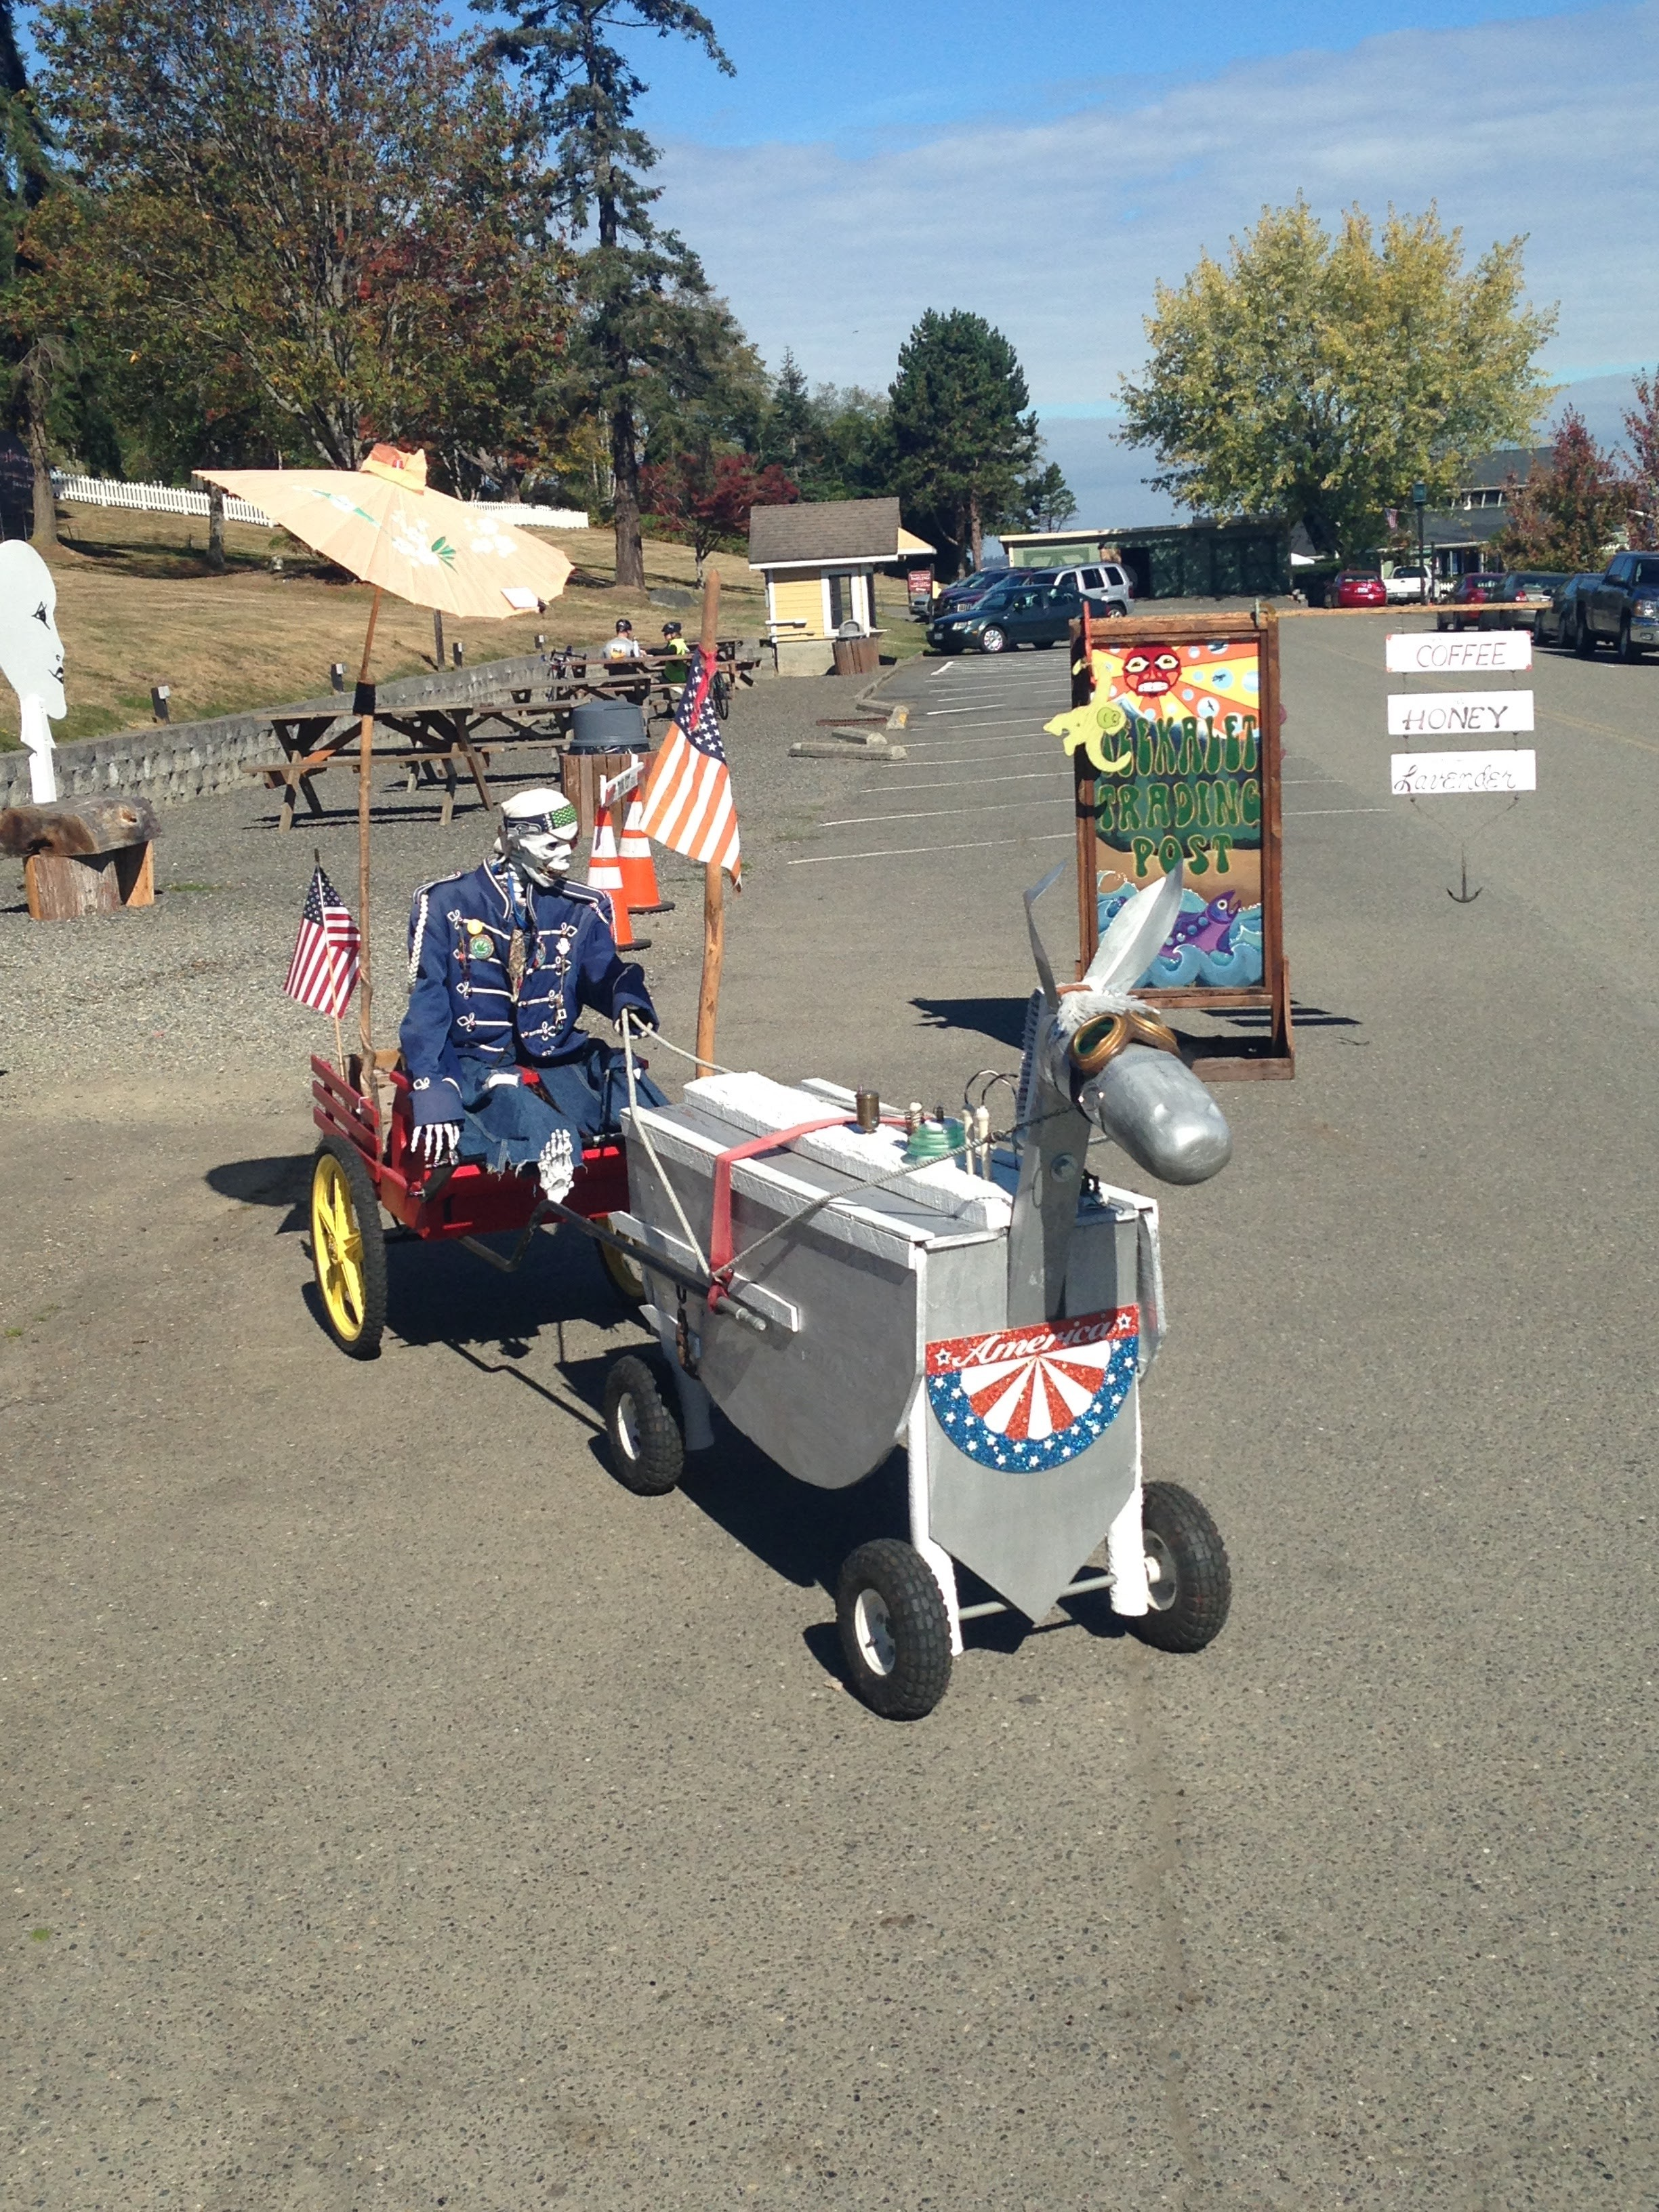
\includegraphics[width=6cm]{/home/paul/Dropbox/MARES_PhD/jointprod_study/docs/paper_headers/IMG_2025}
}
%%%%%%%%%%%%%%%%%%%%%%%%%%%%%%%%%%%%%%%%%%%%%%%%
%%%%%%%%%%%%%%%%%%%%%%%%%%%%%%%%%%%%%%%%%%%%%%%%
\end{document}
%%%%%%%%%%%%%%%%%%%%%%%%%%%%%%%%%%%%%%%%%%%%%%%%
